\documentclass[tikz]{standalone}
\usetikzlibrary{calc}
\usetikzlibrary{decorations.markings,decorations.pathreplacing}
\tikzset{
  % style to apply some styles to each segment of a path
  on each segment/.style={
    decorate,
    decoration={
      show path construction,
      moveto code={},
      lineto code={
        \path [#1]
        (\tikzinputsegmentfirst) -- (\tikzinputsegmentlast);
      },
      curveto code={
        \path [#1] (\tikzinputsegmentfirst)
        .. controls
        (\tikzinputsegmentsupporta) and (\tikzinputsegmentsupportb)
        ..
        (\tikzinputsegmentlast);
      },
      closepath code={
        \path [#1]
        (\tikzinputsegmentfirst) -- (\tikzinputsegmentlast);
      },
    },
  },
  % style to add an arrow in the middle of a path
  mid arrow/.style={postaction={decorate,decoration={
        markings,
        mark=at position .5 with {\arrow[#1]{stealth}}
      }}},
}


\begin{document}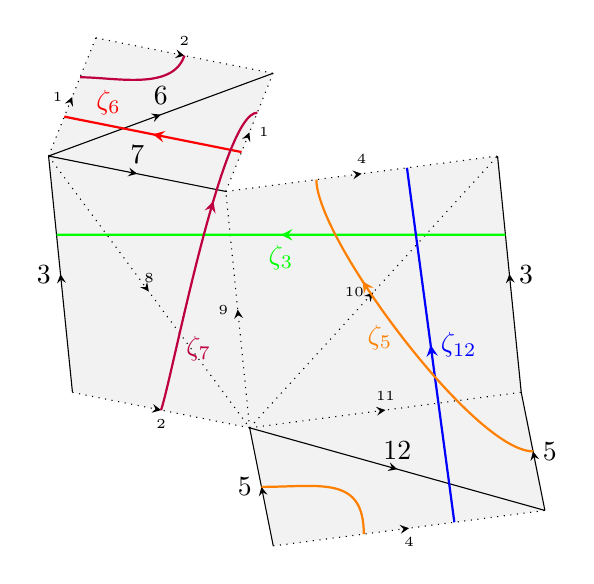
\begin{tikzpicture}[scale=1.5]

\coordinate (z) at (0,0);
\coordinate (v1) at (.4, 1);
\coordinate (v2) at (1.5, -.3);
\coordinate (v3) at (-.2, 2);
\coordinate (v4) at (2.3, .3);
\coordinate (v5) at (-.2, 1);
\coordinate (v6) at ($(z)-(v1)-(v2)$);

\coordinate (x0) at (0,0);
\coordinate (x1) at ($(x0) + (v1)$);
\coordinate (x2) at ($(x1) + (v2)$);
\coordinate (x3) at ($(x2) - (v1)$);
\coordinate (x4) at ($(x3) + (v4)$);
\coordinate (x5) at ($(x4) - (v3)$);
\coordinate (x6) at ($(x5) - (v5)$);
\coordinate (x7) at ($(x6) - (v4)$);
\coordinate (x8) at ($(x7) + (v5)$);
\coordinate (x9) at ($(x8) - (v2)$);
\coordinate (x10) at ($(x9) + (v3)$);

\fill[fill=gray!10] (x0) -- (x1) -- (x2) -- (x3) -- (x4) -- (x5) -- (x6) -- (x7) -- (x8) -- (x9) -- (x10) -- cycle;

\path [draw=black,postaction={on each segment={mid arrow=black}}]
 (x5) -- node[right] {3} (x4)
 (x6) -- node[right] {5} (x5)
 (x7) -- node[left] {5} (x8)
 (x9) -- node[left] {3} (x0)
 (x8) -- node [above] {12} (x6)
 (x0) -- node[above] {6} (x2)
 (x0) -- node[above] {7} (x3);

\path [draw=black,dotted,postaction={on each segment={mid arrow=black}}]
 (x0) -- node[left] {\tiny 1} (x1)
 (x3) -- node[right] {\tiny 1} (x2)
 (x1) -- node[above] {\tiny 2} (x2)
 (x9) -- node[below] {\tiny 2} (x8)
 (x3) -- node[above] {\tiny 4} (x4)
 (x7) -- node[below] {\tiny 4} (x6)
 (x0) -- node [above] {\tiny 8} (x8)
 (x8) -- node [left] {\tiny 9} (x3)
 (x8) -- node [left] {\tiny 10} (x4)
 (x8) -- node [above] {\tiny 11} (x5);

\begin{scope}[thick]
\draw[green,postaction={mid arrow}]  (barycentric cs:x4=2,x5=1) -- node[below] {$\zeta_3$} (barycentric cs:x0=2,x9=1);
\draw [red,postaction={mid arrow}] (barycentric cs:x2=1,x3=2) -- node[above,near end] {$\zeta_6$}  (barycentric cs:x0=2,x1=1) ;
\draw[blue,postaction={mid arrow}] (barycentric cs:x6=2,x7=1) -- node[right] {$\zeta_{12}$} (barycentric cs:x3=1,x4=2);
% zeta5
\draw[orange,postaction={mid arrow}] (barycentric cs:x5=1,x6=1) .. controls +(-.5,0) and +(0,-.5) .. 
node [left] {$\zeta_5$} (barycentric cs:x3=2,x4=1)
(barycentric cs:x6=1,x7=2) .. controls +(0,.5) and +(.5,0) .. (barycentric cs:x7=1,x8=1);

% zeta7
\draw[purple,postaction={mid arrow}] 
 (barycentric cs:x8=1,x9=1) .. controls +(.1,.3) and +(-.3,0) .. node[right,near start] {$\zeta_7$} (barycentric cs:x2=2,x3=1)
 (barycentric cs:x0=1,x1=2) .. controls +(.3,0) and +(-.1,-.3) .. (barycentric cs:x1=1,x2=1);
\end{scope}



\end{tikzpicture}\end{document}
